% Created by tikzDevice version 0.12.6 on 2024-10-30 10:03:09
% !TEX encoding = UTF-8 Unicode
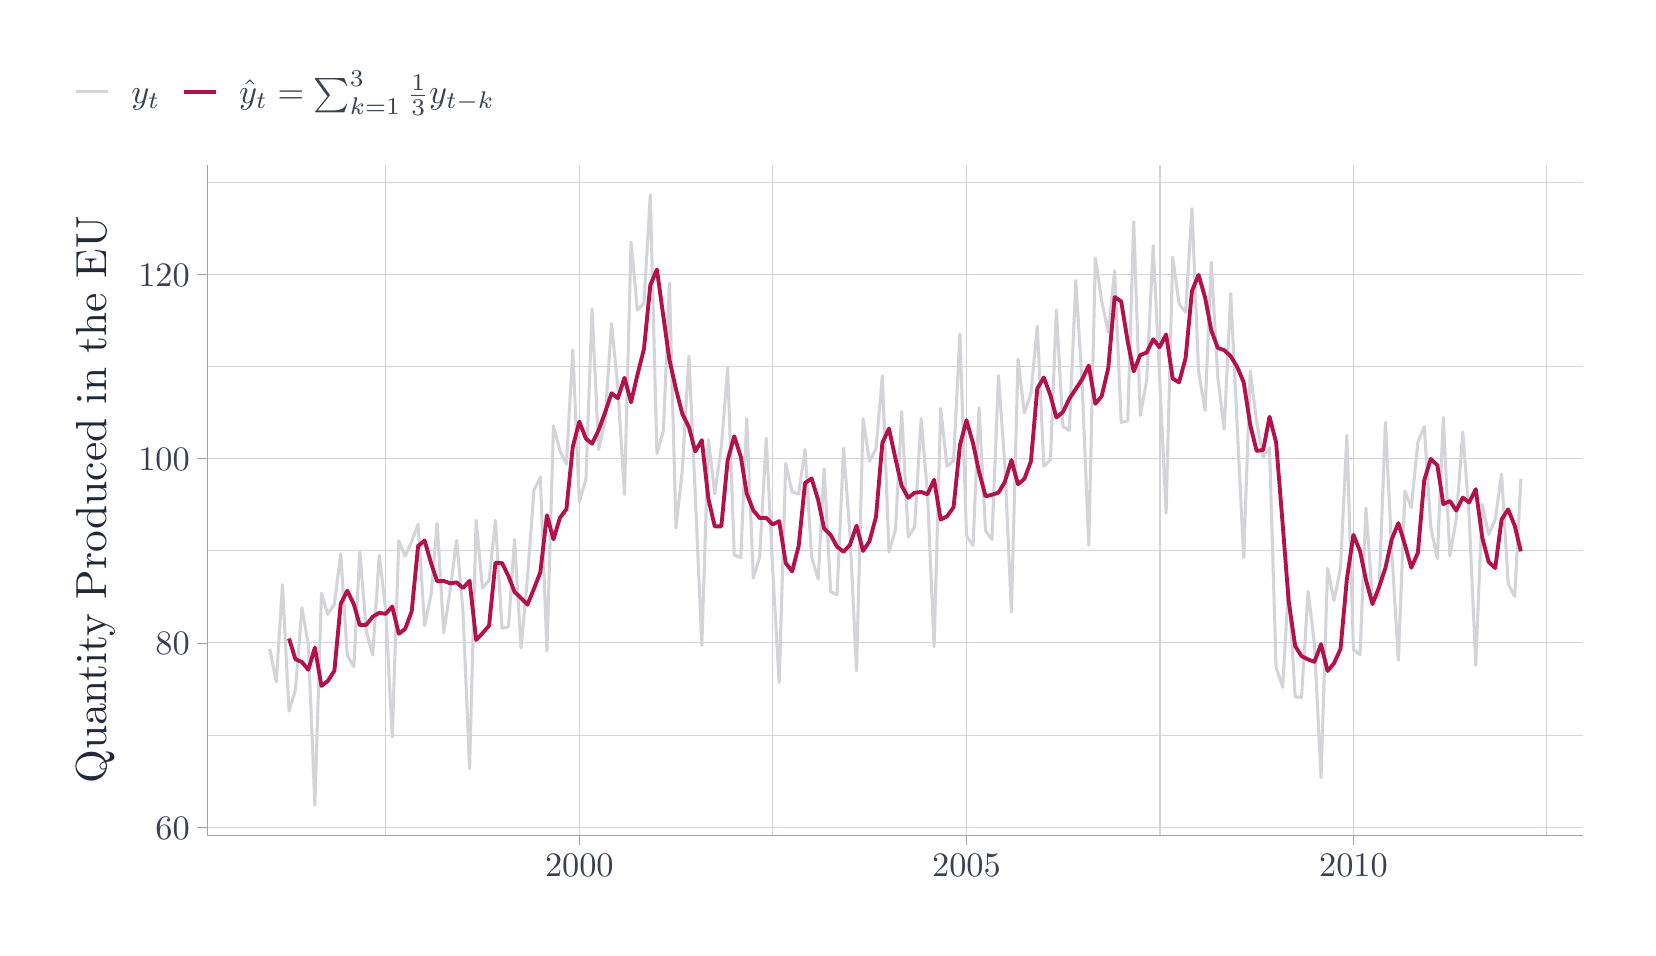
\begin{tikzpicture}[x=1pt,y=1pt]
\definecolor{fillColor}{RGB}{255,255,255}
\path[use as bounding box,fill=fillColor] (0,0) rectangle (578.16,325.21);
\begin{scope}
\path[clip] (  0.00,  0.00) rectangle (578.16,325.21);
\definecolor{drawColor}{RGB}{255,255,255}

\path[draw=drawColor,line width= 0.7pt,line join=round,line cap=round,fill=fillColor] (  0.00,  0.00) rectangle (578.16,325.21);
\end{scope}
\begin{scope}
\path[clip] ( 64.86, 33.29) rectangle (562.16,275.76);
\definecolor{drawColor}{RGB}{255,255,255}
\definecolor{fillColor}{RGB}{255,255,255}

\path[draw=drawColor,line width= 0.7pt,line join=round,line cap=round,fill=fillColor] ( 64.86, 33.29) rectangle (562.16,275.76);
\definecolor{drawColor}{RGB}{209,213,219}

\path[draw=drawColor,line width= 0.4pt,line join=round] ( 64.86, 69.58) --
	(562.16, 69.58);

\path[draw=drawColor,line width= 0.4pt,line join=round] ( 64.86,136.18) --
	(562.16,136.18);

\path[draw=drawColor,line width= 0.4pt,line join=round] ( 64.86,202.77) --
	(562.16,202.77);

\path[draw=drawColor,line width= 0.4pt,line join=round] ( 64.86,269.37) --
	(562.16,269.37);

\path[draw=drawColor,line width= 0.4pt,line join=round] (129.43, 33.29) --
	(129.43,275.76);

\path[draw=drawColor,line width= 0.4pt,line join=round] (269.29, 33.29) --
	(269.29,275.76);

\path[draw=drawColor,line width= 0.4pt,line join=round] (409.15, 33.29) --
	(409.15,275.76);

\path[draw=drawColor,line width= 0.4pt,line join=round] (548.97, 33.29) --
	(548.97,275.76);

\path[draw=drawColor,line width= 0.4pt,line join=round] ( 64.86, 36.28) --
	(562.16, 36.28);

\path[draw=drawColor,line width= 0.4pt,line join=round] ( 64.86,102.88) --
	(562.16,102.88);

\path[draw=drawColor,line width= 0.4pt,line join=round] ( 64.86,169.47) --
	(562.16,169.47);

\path[draw=drawColor,line width= 0.4pt,line join=round] ( 64.86,236.07) --
	(562.16,236.07);

\path[draw=drawColor,line width= 0.4pt,line join=round] (199.34, 33.29) --
	(199.34,275.76);

\path[draw=drawColor,line width= 0.4pt,line join=round] (339.24, 33.29) --
	(339.24,275.76);

\path[draw=drawColor,line width= 0.4pt,line join=round] (479.06, 33.29) --
	(479.06,275.76);
\definecolor{drawColor}{RGB}{212,212,216}

\path[draw=drawColor,line width= 1.1pt,line join=round] ( 87.47,100.71) --
	( 89.84, 88.83) --
	( 92.06,123.92) --
	( 94.44, 78.24) --
	( 96.73, 85.76) --
	( 99.11,115.57) --
	(101.41,102.21) --
	(103.78, 44.31) --
	(106.15,120.89) --
	(108.45,113.23) --
	(110.82,116.90) --
	(113.12,135.18) --
	(115.49, 98.35) --
	(117.87, 94.29) --
	(120.01,135.71) --
	(122.39,107.11) --
	(124.68, 98.48) --
	(127.06,134.54) --
	(129.35,115.10) --
	(131.73, 68.91) --
	(134.10,139.81) --
	(136.40,134.28) --
	(138.77,139.64) --
	(141.07,145.73) --
	(143.44,109.11) --
	(145.82,120.73) --
	(147.96,146.10) --
	(150.34,106.51) --
	(152.63,121.66) --
	(155.01,139.97) --
	(157.30,114.40) --
	(159.68, 57.49) --
	(162.05,147.30) --
	(164.35,122.62) --
	(166.72,125.55) --
	(169.02,147.16) --
	(171.39,108.17) --
	(173.77,108.77) --
	(175.91,140.31) --
	(178.28,101.05) --
	(180.58,126.15) --
	(182.96,158.15) --
	(185.25,162.78) --
	(187.63, 99.98) --
	(190.00,181.33) --
	(192.30,172.44) --
	(194.67,167.48) --
	(196.97,208.77) --
	(199.34,153.82) --
	(201.72,162.05) --
	(203.94,223.52) --
	(206.31,172.74) --
	(208.61,183.03) --
	(210.98,218.22) --
	(213.28,194.85) --
	(215.65,156.55) --
	(218.03,247.72) --
	(220.32,223.15) --
	(222.70,225.61) --
	(224.99,264.74) --
	(227.37,171.34) --
	(229.74,179.63) --
	(231.89,232.94) --
	(234.26,144.37) --
	(236.56,165.31) --
	(238.93,206.57) --
	(241.23,156.59) --
	(243.60,101.95) --
	(245.97,176.37) --
	(248.27,156.75) --
	(250.65,173.67) --
	(252.94,202.27) --
	(255.32,134.58) --
	(257.69,133.75) --
	(259.83,183.96) --
	(262.21,126.35) --
	(264.51,133.95) --
	(266.88,176.80) --
	(269.18,129.95) --
	(271.55, 88.49) --
	(273.92,167.74) --
	(276.22,157.49) --
	(278.60,156.69) --
	(280.89,172.80) --
	(283.27,133.98) --
	(285.64,125.89) --
	(287.78,165.81) --
	(290.16,121.33) --
	(292.45,120.36) --
	(294.83,173.27) --
	(297.13,142.17) --
	(299.50, 92.82) --
	(301.87,183.89) --
	(304.17,168.54) --
	(306.54,173.00) --
	(308.84,199.44) --
	(311.22,135.78) --
	(313.59,143.73) --
	(315.81,186.49) --
	(318.18,141.17) --
	(320.48,144.70) --
	(322.85,183.96) --
	(325.15,156.85) --
	(327.53,101.48) --
	(329.90,187.55) --
	(332.20,166.74) --
	(334.57,168.71) --
	(336.87,214.59) --
	(339.24,141.67) --
	(341.61,138.04) --
	(343.76,187.85) --
	(346.13,143.44) --
	(348.43,140.24) --
	(350.80,199.58) --
	(353.10,167.01) --
	(355.47,114.07) --
	(357.85,205.44) --
	(360.15,185.96) --
	(362.52,193.02) --
	(364.82,217.42) --
	(367.19,166.68) --
	(369.56,169.01) --
	(371.71,223.22) --
	(374.08,181.06) --
	(376.38,179.70) --
	(378.75,233.81) --
	(381.05,195.91) --
	(383.42,138.14) --
	(385.80,242.06) --
	(388.09,226.45) --
	(390.47,215.13) --
	(392.77,237.30) --
	(395.14,182.56) --
	(397.51,183.13) --
	(399.66,255.12) --
	(402.03,185.12) --
	(404.33,197.61) --
	(406.70,246.43) --
	(409.00,199.08) --
	(411.37,149.73) --
	(413.75,242.33) --
	(416.04,225.45) --
	(418.42,222.32) --
	(420.71,259.84) --
	(423.09,200.94) --
	(425.46,186.89) --
	(427.68,240.47) --
	(430.06,198.71) --
	(432.35,180.13) --
	(434.73,229.18) --
	(437.02,181.99) --
	(439.40,133.75) --
	(441.77,201.11) --
	(444.07,182.86) --
	(446.44,169.87) --
	(448.74,173.40) --
	(451.11, 94.15) --
	(453.49, 86.86) --
	(455.63,124.19) --
	(458.01, 83.33) --
	(460.30, 83.23) --
	(462.68,121.56) --
	(464.97,102.55) --
	(467.35, 54.13) --
	(469.72,129.82) --
	(472.02,118.20) --
	(474.39,129.82) --
	(476.69,177.87) --
	(479.06,100.48) --
	(481.44, 98.68) --
	(483.58,151.56) --
	(485.95,118.40) --
	(488.25,120.19) --
	(490.63,182.59) --
	(492.92,135.74) --
	(495.30, 96.69) --
	(497.67,157.82) --
	(499.97,151.76) --
	(502.34,175.37) --
	(504.64,181.06) --
	(507.01,144.73) --
	(509.39,133.38) --
	(511.53,184.39) --
	(513.90,134.34) --
	(516.20,147.50) --
	(518.57,179.13) --
	(520.87,148.73) --
	(523.25, 94.82) --
	(525.62,152.96) --
	(527.92,142.07) --
	(530.29,147.40) --
	(532.59,163.95) --
	(534.96,124.32) --
	(537.34,119.66) --
	(539.56,162.15);
\definecolor{drawColor}{RGB}{179,17,75}

\path[draw=drawColor,line width= 1.4pt,line join=round] ( 94.44,104.49) --
	( 96.73, 97.00) --
	( 99.11, 95.97) --
	(101.41, 93.19) --
	(103.78,101.18) --
	(106.15, 87.36) --
	(108.45, 89.14) --
	(110.82, 92.81) --
	(113.12,117.01) --
	(115.49,121.77) --
	(117.87,116.81) --
	(120.01,109.27) --
	(122.39,109.45) --
	(124.68,112.37) --
	(127.06,113.77) --
	(129.35,113.38) --
	(131.73,116.04) --
	(134.10,106.19) --
	(136.40,107.94) --
	(138.77,114.33) --
	(141.07,137.91) --
	(143.44,139.88) --
	(145.82,131.49) --
	(147.96,125.19) --
	(150.34,125.31) --
	(152.63,124.44) --
	(155.01,124.76) --
	(157.30,122.71) --
	(159.68,125.34) --
	(162.05,103.96) --
	(164.35,106.40) --
	(166.72,109.14) --
	(169.02,131.83) --
	(171.39,131.78) --
	(173.77,126.96) --
	(175.91,121.37) --
	(178.28,119.08) --
	(180.58,116.71) --
	(182.96,122.50) --
	(185.25,128.45) --
	(187.63,149.03) --
	(190.00,140.31) --
	(192.30,148.03) --
	(194.67,151.25) --
	(196.97,173.75) --
	(199.34,182.89) --
	(201.72,176.69) --
	(203.94,174.88) --
	(206.31,179.80) --
	(208.61,186.10) --
	(210.98,193.09) --
	(213.28,191.33) --
	(215.65,198.70) --
	(218.03,189.87) --
	(220.32,199.71) --
	(222.70,209.14) --
	(224.99,232.16) --
	(227.37,237.83) --
	(229.74,220.56) --
	(231.89,205.24) --
	(234.26,194.64) --
	(236.56,185.65) --
	(238.93,180.87) --
	(241.23,172.08) --
	(243.60,176.16) --
	(245.97,155.03) --
	(248.27,144.97) --
	(250.65,145.02) --
	(252.94,168.93) --
	(255.32,177.57) --
	(257.69,170.17) --
	(259.83,156.87) --
	(262.21,150.76) --
	(264.51,148.02) --
	(266.88,148.09) --
	(269.18,145.70) --
	(271.55,146.90) --
	(273.92,131.75) --
	(276.22,128.73) --
	(278.60,137.91) --
	(280.89,160.64) --
	(283.27,162.33) --
	(285.64,154.49) --
	(287.78,144.22) --
	(290.16,141.89) --
	(292.45,137.67) --
	(294.83,135.83) --
	(297.13,138.32) --
	(299.50,145.27) --
	(301.87,136.09) --
	(304.17,139.63) --
	(306.54,148.42) --
	(308.84,175.15) --
	(311.22,180.33) --
	(313.59,169.41) --
	(315.81,159.65) --
	(318.18,155.33) --
	(320.48,157.13) --
	(322.85,157.45) --
	(325.15,156.61) --
	(327.53,161.84) --
	(329.90,147.43) --
	(332.20,148.63) --
	(334.57,151.93) --
	(336.87,174.34) --
	(339.24,183.35) --
	(341.61,174.99) --
	(343.76,164.77) --
	(346.13,155.86) --
	(348.43,156.44) --
	(350.80,157.18) --
	(353.10,161.08) --
	(355.47,168.94) --
	(357.85,160.22) --
	(360.15,162.17) --
	(362.52,168.49) --
	(364.82,194.80) --
	(367.19,198.80) --
	(369.56,192.37) --
	(371.71,184.37) --
	(374.08,186.30) --
	(376.38,191.10) --
	(378.75,194.66) --
	(381.05,198.19) --
	(383.42,203.14) --
	(385.80,189.29) --
	(388.09,192.04) --
	(390.47,202.22) --
	(392.77,227.88) --
	(395.14,226.29) --
	(397.51,211.66) --
	(399.66,201.00) --
	(402.03,206.93) --
	(404.33,207.79) --
	(406.70,212.62) --
	(409.00,209.72) --
	(411.37,214.37) --
	(413.75,198.41) --
	(416.04,197.04) --
	(418.42,205.84) --
	(420.71,230.03) --
	(423.09,235.87) --
	(425.46,227.70) --
	(427.68,215.89) --
	(430.06,209.43) --
	(432.35,208.69) --
	(434.73,206.43) --
	(437.02,202.67) --
	(439.40,197.10) --
	(441.77,181.64) --
	(444.07,172.28) --
	(446.44,172.57) --
	(448.74,184.61) --
	(451.11,175.38) --
	(453.49,145.81) --
	(455.63,118.14) --
	(458.01,101.74) --
	(460.30, 98.13) --
	(462.68, 96.92) --
	(464.97, 96.04) --
	(467.35,102.45) --
	(469.72, 92.74) --
	(472.02, 95.50) --
	(474.39,100.71) --
	(476.69,125.94) --
	(479.06,141.96) --
	(481.44,136.05) --
	(483.58,125.68) --
	(485.95,116.91) --
	(488.25,122.88) --
	(490.63,130.05) --
	(492.92,140.39) --
	(495.30,146.18) --
	(497.67,138.34) --
	(499.97,130.08) --
	(502.34,135.42) --
	(504.64,161.65) --
	(507.01,169.40) --
	(509.39,167.05) --
	(511.53,153.06) --
	(513.90,154.17) --
	(516.20,150.71) --
	(518.57,155.41) --
	(520.87,153.66) --
	(523.25,158.45) --
	(525.62,140.89) --
	(527.92,132.17) --
	(530.29,129.95) --
	(532.59,147.48) --
	(534.96,151.14) --
	(537.34,145.22) --
	(539.56,135.98);
\end{scope}
\begin{scope}
\path[clip] (  0.00,  0.00) rectangle (578.16,325.21);
\definecolor{drawColor}{RGB}{156,163,175}

\path[draw=drawColor,line width= 0.3pt,line join=round] ( 64.86, 33.29) --
	( 64.86,275.76);
\end{scope}
\begin{scope}
\path[clip] (  0.00,  0.00) rectangle (578.16,325.21);
\definecolor{drawColor}{RGB}{55,65,81}

\node[text=drawColor,anchor=base east,inner sep=0pt, outer sep=0pt, scale=  1.24] at ( 58.56, 32.00) {60};

\node[text=drawColor,anchor=base east,inner sep=0pt, outer sep=0pt, scale=  1.24] at ( 58.56, 98.59) {80};

\node[text=drawColor,anchor=base east,inner sep=0pt, outer sep=0pt, scale=  1.24] at ( 58.56,165.19) {100};

\node[text=drawColor,anchor=base east,inner sep=0pt, outer sep=0pt, scale=  1.24] at ( 58.56,231.79) {120};
\end{scope}
\begin{scope}
\path[clip] (  0.00,  0.00) rectangle (578.16,325.21);
\definecolor{drawColor}{RGB}{156,163,175}

\path[draw=drawColor,line width= 0.3pt,line join=round] ( 61.36, 36.28) --
	( 64.86, 36.28);

\path[draw=drawColor,line width= 0.3pt,line join=round] ( 61.36,102.88) --
	( 64.86,102.88);

\path[draw=drawColor,line width= 0.3pt,line join=round] ( 61.36,169.47) --
	( 64.86,169.47);

\path[draw=drawColor,line width= 0.3pt,line join=round] ( 61.36,236.07) --
	( 64.86,236.07);
\end{scope}
\begin{scope}
\path[clip] (  0.00,  0.00) rectangle (578.16,325.21);
\definecolor{drawColor}{RGB}{156,163,175}

\path[draw=drawColor,line width= 0.3pt,line join=round] ( 64.86, 33.29) --
	(562.16, 33.29);
\end{scope}
\begin{scope}
\path[clip] (  0.00,  0.00) rectangle (578.16,325.21);
\definecolor{drawColor}{RGB}{156,163,175}

\path[draw=drawColor,line width= 0.3pt,line join=round] (199.34, 29.79) --
	(199.34, 33.29);

\path[draw=drawColor,line width= 0.3pt,line join=round] (339.24, 29.79) --
	(339.24, 33.29);

\path[draw=drawColor,line width= 0.3pt,line join=round] (479.06, 29.79) --
	(479.06, 33.29);
\end{scope}
\begin{scope}
\path[clip] (  0.00,  0.00) rectangle (578.16,325.21);
\definecolor{drawColor}{RGB}{55,65,81}

\node[text=drawColor,anchor=base,inner sep=0pt, outer sep=0pt, scale=  1.24] at (199.34, 18.42) {2000};

\node[text=drawColor,anchor=base,inner sep=0pt, outer sep=0pt, scale=  1.24] at (339.24, 18.42) {2005};

\node[text=drawColor,anchor=base,inner sep=0pt, outer sep=0pt, scale=  1.24] at (479.06, 18.42) {2010};
\end{scope}
\begin{scope}
\path[clip] (  0.00,  0.00) rectangle (578.16,325.21);
\definecolor{drawColor}{RGB}{31,41,55}

\node[text=drawColor,rotate= 90.00,anchor=base,inner sep=0pt, outer sep=0pt, scale=  1.57] at ( 28.38,154.52) {Quantity Produced in the EU};
\end{scope}
\begin{scope}
\path[clip] (  0.00,  0.00) rectangle (578.16,325.21);
\definecolor{drawColor}{RGB}{255,255,255}
\definecolor{fillColor}{RGB}{255,255,255}

\path[draw=drawColor,line width= 0.7pt,line join=round,line cap=round,fill=fillColor] ( 16.00,289.76) rectangle (169.07,309.22);
\end{scope}
\begin{scope}
\path[clip] (  0.00,  0.00) rectangle (578.16,325.21);
\definecolor{drawColor}{RGB}{255,255,255}
\definecolor{fillColor}{RGB}{255,255,255}

\path[draw=drawColor,line width= 0.7pt,line join=round,line cap=round,fill=fillColor] ( 16.00,294.76) rectangle ( 30.45,309.22);
\end{scope}
\begin{scope}
\path[clip] (  0.00,  0.00) rectangle (578.16,325.21);
\definecolor{drawColor}{RGB}{212,212,216}

\path[draw=drawColor,line width= 1.1pt,line join=round] ( 17.45,301.99) -- ( 29.01,301.99);
\end{scope}
\begin{scope}
\path[clip] (  0.00,  0.00) rectangle (578.16,325.21);
\definecolor{drawColor}{RGB}{255,255,255}
\definecolor{fillColor}{RGB}{255,255,255}

\path[draw=drawColor,line width= 0.7pt,line join=round,line cap=round,fill=fillColor] ( 54.93,294.76) rectangle ( 69.39,309.22);
\end{scope}
\begin{scope}
\path[clip] (  0.00,  0.00) rectangle (578.16,325.21);
\definecolor{drawColor}{RGB}{179,17,75}

\path[draw=drawColor,line width= 1.4pt,line join=round] ( 56.38,301.99) -- ( 67.94,301.99);
\end{scope}
\begin{scope}
\path[clip] (  0.00,  0.00) rectangle (578.16,325.21);
\definecolor{drawColor}{RGB}{55,65,81}

\node[text=drawColor,anchor=base west,inner sep=0pt, outer sep=0pt, scale=  1.24] at ( 37.45,297.70) {$y_t$};
\end{scope}
\begin{scope}
\path[clip] (  0.00,  0.00) rectangle (578.16,325.21);
\definecolor{drawColor}{RGB}{55,65,81}

\node[text=drawColor,anchor=base west,inner sep=0pt, outer sep=0pt, scale=  1.24] at ( 76.39,297.70) {$\hat{y}_t = \sum_{k=1}^3 \frac{1}{3} y_{t-k}$};
\end{scope}
\end{tikzpicture}
